\documentclass[11pt, tikz]{standalone}
\usepackage[T1]{fontenc}
\usepackage[utf8]{inputenc}
%\usepackage{textcomp}
%\renewcommand{\ttdefault}{lmtt} % 
\usepackage{amsmath}
\usetikzlibrary{arrows.meta, decorations.pathmorphing, positioning, calc}
\usepackage{xcolor}

\begin{document}\sffamily
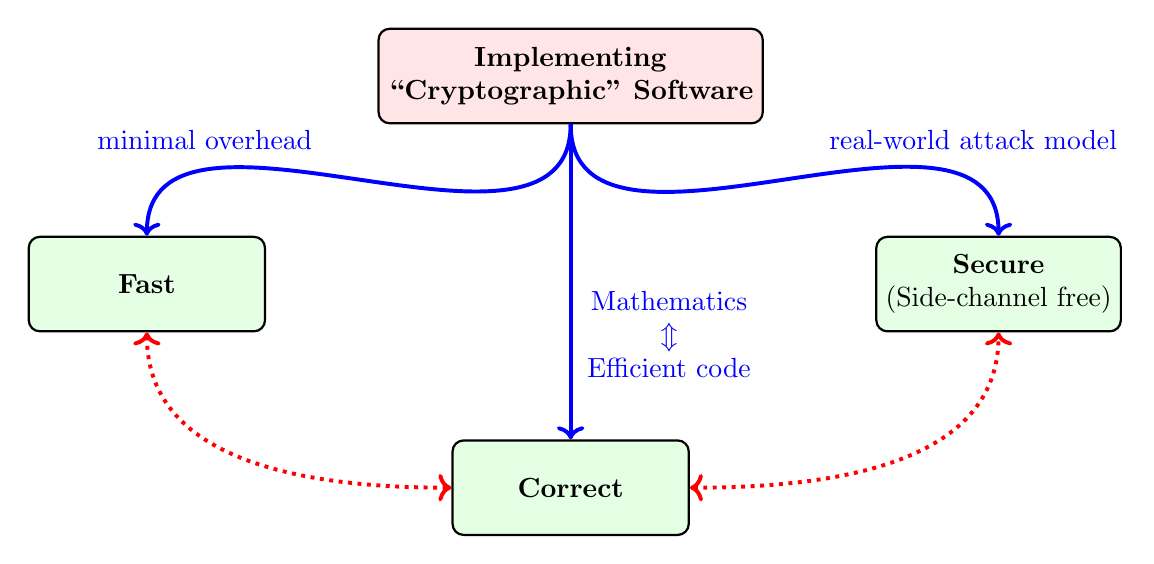
\begin{tikzpicture}[
	bluebox/.style={rectangle, draw, thick, rounded corners, minimum height=1.2cm, minimum width=2.5cm, align=center, fill=blue!10},
	yellowbox/.style={rectangle, draw, thick, rounded corners, minimum height=1.2cm, minimum width=2.5cm, align=center, fill=yellow!10},
	greenbox/.style={rectangle, draw, thick, rounded corners, minimum height=1.2cm, minimum width=3cm, align=center, fill=green!10},
	redbox/.style={rectangle, draw, thick, rounded corners, minimum height=1.2cm, minimum width=3cm, align=center, fill=red!10},
	arrow/.style={->, line width=.5mm},
	every node/.style={align=center}
	]
	\node[redbox] (crypto-sw) {\textbf{Implementing}\\ \textbf{``Cryptographic'' Software}};
	\node[greenbox, below left=2cm of crypto-sw] (ef) {\bfseries Fast};
	\node[greenbox, below=4cm of crypto-sw] (fc) {\bfseries Correct};
	\node[greenbox, below right=2cm of crypto-sw] (sca) {\bfseries Secure\\ (Side-channel free)};
	\draw[arrow, blue, out=-90, in=90] (crypto-sw) to (ef);
	\node[blue, below left=1cm of crypto-sw, yshift=.75cm] () {minimal overhead};
	\draw[arrow, blue, out=-90, in=90] (crypto-sw) to (sca);
	\node[blue, below=2cm of crypto-sw, xshift=1.25cm] () {Mathematics\\$\Updownarrow$ \\Efficient code};
	\draw[arrow, blue, out=-90, in=90] (crypto-sw) to (fc);
	\node[blue, below right=1cm of crypto-sw, yshift=.75cm] () {real-world attack model};
	
	\draw[dotted, <->, line width=.5mm, red, out=-90, in=180] (ef) to (fc);
	\draw[dotted, <->, line width=.5mm, red, out=0, in=-90] (fc) to (sca);
\end{tikzpicture}
\end{document}
